\title{INTD262: Number Systems in pre-Columbian Mayan Culture}
\author{Dr. Jordan Hanson - Whittier College Dept. of Physics and Astronomy}
\date{\today}
\documentclass[12pt]{article}
\usepackage[margin=1.5cm]{geometry}
\usepackage{hyperref}
\usepackage{graphicx}
\usepackage{amsmath}
\begin{document}
\maketitle

\section{Introduction}

In this activity, we will learn that written numbers are actually symbols within a larger system, and that other systems exist.  We will learn that the symbols correspond to abstract ideas that appear to be universal to human beings.  We will introduce the concepts of \textit{digits} and \textit{weights}, and four systems that use them to form numbers.  First, we will understand the binary system, arguably the simplest number system.  Second, we already understand the base-10 or Hindu-Arabic system.  Third, we will understand the base-16 or hexadecimal system.  Fourth, we will explore the base-20 or vigesimal system.  Finally, we will apply our knowledge of the vigesimal system to perform calculations as the Mayans did.

\section{Digits and Bases}

Consider the number 255.  You may have learned how to break this type of number into \textit{digits} and \textit{weights}.  There are three digits: one ``2,'' and two instances of ``5.''  What do the digits mean, given that they are not in the same location?  We know the answer from basic math courses:
\begin{equation}
255 = 2\times 100 + 5\times 10 + 5\times 1 = 2\times 10^2 + 5\times 10^1 + 5\times 10^0
\end{equation}
The left/right position of the digits determines how much \textit{weight} we give each digit.  For example, the 2 has a \textit{weight} of 100, or $10^2$.  The first 5 has a \textit{weight} of 10, or $10^1$.  The final five has a \textit{weight} of 1, or $10^0$.  The fact that the weights use powers of 10 reveals that we are using a \textit{base-10} number system.  Switching the base of our number system requires us to think on a level that resembles switching our \textit{language} that we use to speak.  Though we may grasp an idea in our mind, communicating it becomes challenging because we've changed the underlying set of symbols used to communicate.  Consider the following examples, as we switch to base-2 (\textit{binary}).

\section{Base-2 or Binary}

\begin{itemize}
\item Consider the numbers 255 and 256.  Can you identify the power of 2 that corresponds to 256?  Powers of two grow like this: 1, 2, 4, 8, 16, 32, ... ($2^0$, $2^1$, $2^2$, $2^3$, $2^4$, $2^5$). \\ \vspace{1cm}
\item Try obtaining the power of 2: (a) 512 (b) 1024 (c) 2048. \\ \vspace{1cm} 
\item Binary works with just two digits: 0 and 1.  The number of digits is the same as the base.  For the number nine, all we have to do is put a 1 in the 8's place, and add 1: $1001 = 1000 + 1$.  Convert the following \textit{decimal} numbers into binary: (a) 5 (b) 17 (c) 33. \\ \vspace{1.5cm}
\item Now write 256 in binary.  Recall that $2^8 = 256$. \\ \vspace{1cm}
\item How do you suppose we write 255 in binary?  Recall that $2^8 = 256$. Consider what you do when you write 19, as opposed to 20.  If we add a 1 to the 9, it becomes 10.  But the 10 is a ``1'' that goes in the ``ten's place.''  There's already a 1 there (19), so the 1's combine to be a 2.  Thus, we get 20.  (a) Try adding a binary 1 to 11.  What is the result?  (b) Now add 1 to 1111.  (c) Repeat with 111111 + 1.  (d) How do you write 255 in binary?  \\ \vspace{2cm}
\end{itemize}

\section{Base-10 or Hindu-Arabic}

The Hindu–Arabic numeral system is a positional, base-10 numeral system.  Our discussion is confined to \textit{integers}, as opposed to \textit{decimals} (fractions of integers and irrational numbers.

The Hindu–Arabic system was invented between the 1st and 4th centuries by mathematicians from India, and later adopted into the Arabic-speaking world by the 9th century. The system had spread to medieval Europe by the High Middle Ages, but was mainly confined to Northern Italy until the evolution of the printing press in the 15th century.

These symbol sets can be divided into three main families: Western Arabic numerals used in the Greater Maghreb and in Europe; Eastern Arabic numerals used in the Middle East; and the Indian numerals in various scripts used in the Indian subcontinent.

\section{Base-16 or Hexadecimal}

A number system that is common in computer programming is hexadecimal.  Hexadecimal is a modern base-16 system that uses the ten digits of the Hindu-Arabic system, plus the letters A-F.  The reason A-F are needed is because we need 16 digits in a base-16 system.  Counting to 16 in hexadecimal looks like this: ``0, 1, 2, ..., 9, A, B, ..., F, 10.''  The letters A through F have the numerical values of 10-15, respectively.  The number 10 in hexadecimal breaks down like this:

\begin{equation}
10 = 16 \times 16^1 + 0 \times 16^0
\end{equation}

A (base-10) 35 converts to hexadecimal like this:

\begin{equation}
23 = 2 \times 16^1 + 3 \times 16^0
\end{equation}

Try to perform the following conversions:

\begin{itemize}
\item Convert 14 from decimal to hexadecimal. \\ \vspace{1cm}
\item Convert 36 from decimal to hexadecimal. \\ \vspace{1cm}
\item Convert 72 from decimal to hexadecimal. \\ \vspace{1cm}
\item Convert 256 from decimal to hexadecimal. \\ \vspace{1cm}
\item Convert 2048 from decimal to hexadecimal. \\ \vspace{1cm}
\end{itemize}

\section{Base-20 or Vigesimal}

It would be a straightforward exercise to modify our hexadecimal system to a vigesimal (base-20) system by adding more letters.  Our final goal, however, is to understand an example of pre-Columbian calculation in Mesoamerica.  First, note that in a base-20 system, the first few powers of 20 are 1 ($20^0$), 20 ($20^1$), and 400 ($20^2$). Thus, the number 111 in vigesimal translates to

\begin{equation}
111 = 1 \times 20^2 + 1\times 20^1 + 1\times 20^0 = 400 + 20 + 1 = 421
\end{equation}

On the right hand side of the equation, we are representing the number in decimal.  Thus, 421 in decimal translates to 111 in binary.

\begin{itemize}
\item Translate the decimal number 3620 into vigesimal. \\ \vspace{1cm}
\item Translate the decimal number 2081 into vigesimal. \\ \vspace{1cm}
\end{itemize}

\clearpage

Now consider Fig. \ref{fig:maya}.  The Maya used a vigesimal system with 20 digits, comprised of three symbols.  A dot represents one unit, and a bar represents five.  The empty shell represents zero.  For example, two bars and four dots represents ``14,'' or $5 + 5 + 4$.  Notice that the digits are constructed vertically.  The two bars in 14 are stacked, and the dots rest on top.  For numbers larger than 20, the digits having a weight of 20 instead of 1 are above the least significant digits.  Digits with a weight of 400 are above those that receive a weight of 20.  Numbers are therefore written vertically.

\begin{figure}
\centering
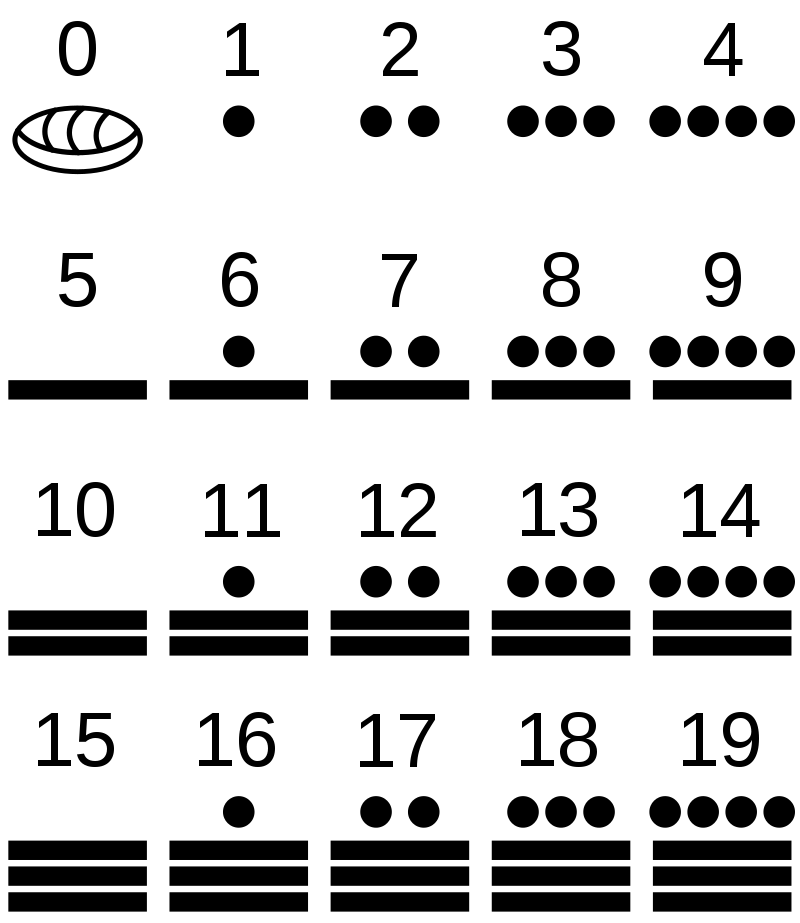
\includegraphics[width=5cm]{figures/maya_digits.png}
\caption{\label{fig:maya} The 20 digits of the Mayan system.  The digit for 0 resembles an empty shell.  The dots are worth 1 and the bars are worth 5.  In a number larger than 19, the symbols stack vertically.}
\end{figure}

Try the following exercises:

\begin{itemize}
\item Write the decimal number 17 using the Mayan script. \\ \vspace{2cm}
\item Write the decimal number 245 using the Mayan script. \\ \vspace{2cm}
\item Write the decimal number 2048 using the Mayan script. \\ \vspace{2cm}
\item Write the decimal number 10000 using the Mayan script. \\ \vspace{2cm}
\end{itemize}

\clearpage

Notice that very large numbers do not require many digits in vigesimal or hexadecimal, owing to the choice of bases.  Now try some addition and subtraction in the Mayan script.

\begin{itemize}
\item (a) Write 25 and 15 in the Mayan script.  Arrange the 25 to the left of the 15.  (b) Now subtract 15 from 25. Note that we must break the dot, which is worth 20, into four bars (each worth 5).  Bar minus bar equals zero, and dot minus dot equals zero. \\ \vspace{2cm}
\item Now add 25 and 15 in the Mayan script.  Note that four bars (four times five) equal one dot, but in the higher positiion. \\ \vspace{2cm}
\item (a) Write the numbers 425 and 675 in the Mayan script.  (b) Add $675 + 425$.  (c) Subtract $675 - 425$.
\end{itemize}

\end{document}
